\documentclass[../main/main.tex]{subfiles}
\graphicspath{{./figures/}}

\makeatletter
\renewcommand{\@chapapp}{Travaux pratiques -- TP}
\renewcommand{\chaplett}{TP}
\makeatother

% \toggletrue{student}
% \toggletrue{corrige}
% \renewcommand{\mycol}{black}
% \renewcommand{\mycol}{gray}

\hfuzz=5.003pt

\begin{document}
\setcounter{chapter}{5}

\settype{enon}
\settype{solu_prof}
\settype{solu_stud}

\chapter{Oscilloscope et trac\'e de caract\'eristiques}

\enonce{
	\begin{tcn}[sidebyside](appl)<ctb>"how"'t'{Capacités exigibles}
		\begin{itemize}[label=\rcheck]
			\item Préciser la perturbation induite par l'appareil de mesure sur le
			      montage et ses limites (bande passante, résistance d'entrée)~;
			\item Définir la nature de la mesure effectuée (valeur efficace, valeur
			      moyenne, amplitude, valeur crête à crête, etc.)~;
			\item Mesurer une tension au voltmètre ou à l'oscilloscope~;
		\end{itemize}
		\tcblower
		\begin{itemize}[label=\rcheck]
			\item Gérer, dans un circuit électronique, les contraintes liées à la
			      liaison entre les masses.
			\item Obtenir un signal de valeur moyenne, de forme, d’amplitude et de
			      fréquence données.
			\item Mettre en œuvre une méthode de mesure de fréquence ou de période.
		\end{itemize}
	\end{tcn}
	\vspace{-10pt}
	\section{Objectifs}
	\begin{itemize}
		\item Se familiariser avec le GBF et l'oscilloscope numérique.
		\item Réaliser des montages simples d'électricité.
		      % \item Mesurer la résistance d'entrée $R_{e}$ d'un oscilloscope et la
		      %       résistance de sortie $R_{s}$ d'un GBF.
		\item Tracer une caractéristique de dipôle en utilisant un transformateur
		      d'isolement.
	\end{itemize}

	\begin{tcn}[cnt, bld](impo){}
		Vous prendrez soin de refaire tous les schémas des circuits mis en place ou
		étudiés.
	\end{tcn}
}

\section{S'approprier}
\subsection{Résistances d'entrée et de sortie}

% Nous avons vu en TD la méthode dite de la «~demi-tension~» qui permet de
% mesurer la résistance d'entrée et de sortie d'un appareil (cf.\ exercice I TD
% 2, fait \textit{via} la puissance)

\subsubsection{Résistance de sortie du générateur basse fréquence (GBF)}

\enonce{%
	\begin{tcb}[sidebyside, righthand ratio=.35](defi){Résistance de sortie}
		Le GBF est un générateur réel pouvant être modélisé comme une association
		série d'un générateur idéal de tension de force électromotrice $e$ associé à
		une résistance de sortie $r_{s}$ (modèle de \textsc{Thévenin}). Comme vu en
		cours, on branche le GBF sur une résistance variable $R'$ puis on mesure la
		tension $U_1$ aux bornes de $R'$.
		\tcblower
		\begin{center}
			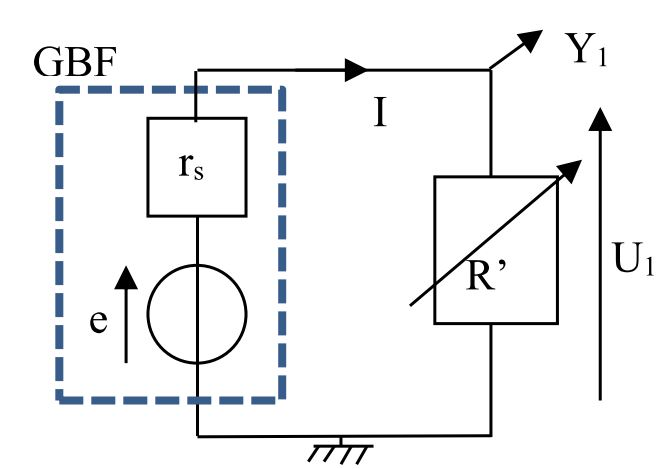
\includegraphics[width=\linewidth]{res_entree}
			\captionof{figure}{}
		\end{center}
	\end{tcb}
}%

\setlist[blocQR,1]{leftmargin=10pt, label=\clenumi}
\QR{%
	Montrer que lorsque $U_1 = e/2$, alors $R' = r_{s}$.
}{%
	Par un pont diviseur de tension,
	\begin{gather*}
		U_1 = \frac{R'}{R'+r_s}e
		\\\beforetext{donc}
		U_1 = \frac{e}{2}
		\Lra
		\frac{R'}{R'+r_s} = \frac{1}{2}
		\Lra
		\boxed{R' = r_s}
	\end{gather*}
}%

\QR{%
	En déduire une méthode simple de mesure expérimentale de $r_{s}$.
}{%
	On mesure la tension à vide du GBF en branchant un voltmètre directement
	dessus. On branche ensuite une résistance variable à ses bornes et le
	voltmètre par-dessus. On fait varier la résistance entre
	\SIrange{1}{100}{\ohm}. Lorsque la tension lue est la moitié de la tension à
	vide, on relève la valeur de $R'$~: c'est la valeur de $r_s$.
}%

\subsubsection{Résistance d'entrée de l'oscilloscope}

\enonce{%
	\begin{tcb}[sidebyside, righthand ratio=.35](defi){Résistance d'entrée}
		L'entrée d'un oscilloscope est assimilable à une résistance d'entrée $R_{e}$
		en dérivation avec une capacité $C_{e}$. À \textbf{basse fréquence}, le
		condensateur est assimilable à un \textbf{interrupteur ouvert}.
		\tcblower
		\begin{center}
			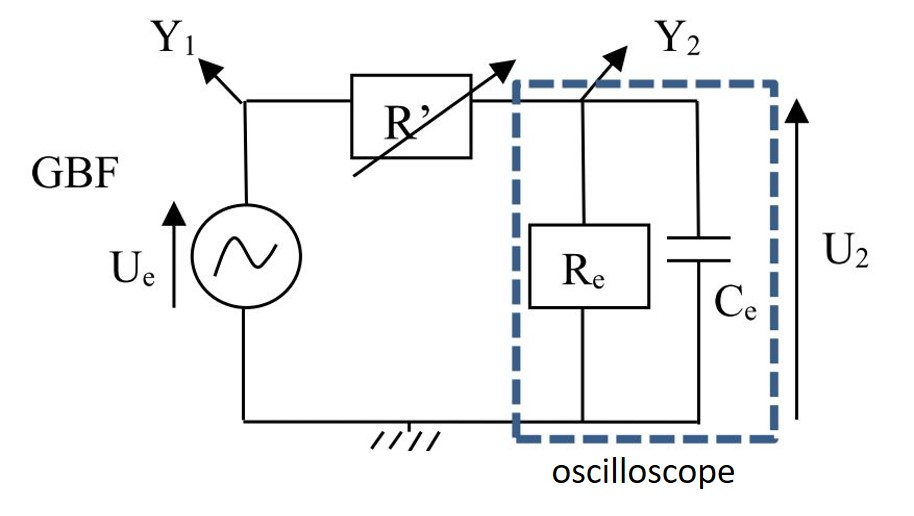
\includegraphics[width=\linewidth]{res_sortie}
			\captionof{figure}{}
		\end{center}
	\end{tcb}

	\begin{tcb}(rema)<lfnt>{}
		Remarquez que, contrairement à ce qui est fait dans le cours, la résistance de
		sortie du GBF n'apparaît pas. Elle est en réalité très faible devant les
		autres résistances $R_{e}$ et $R'$ et sera donc négligée.
	\end{tcb}
}%

\QR{%
	Montrer alors, en vous aidant du schéma, que la tension $U_2$ mesurée
	par l'oscilloscope (modélisée par une résistance et une capacité en
	parallèle) est égale à $U_{e}/2$ lorsque $R' = R_{e}$.
}{%
	Avec $C_e$ un interrupteur ouvert, aucune intensité ne passe dans la branche
	de la capacité. On se retrouve donc avec un autre pont diviseur de tension,
	avec
	\begin{gather*}
		U_2 = \frac{R_e}{R_e + R'}U_e
		\\\beforetext{donc}
		U_2 = \frac{U_e}{2}
		\Lra
		\frac{R_e}{R_e + R'} = \frac{1}{2}
		\Lra
		\boxed{R' = R_e}
	\end{gather*}
}%

\QR{%
	En déduire une méthode simple de mesure expérimentale de $R_{e}$.
}{%
	Avec un $U_e$ connu, par exemple, $U_e = \SI{5}{V}$ constant, on branche
	l'oscilloscope et on oberve la tension mesurée. On fait varier $R'$ jusqu'à ce
	que l'oscilloscope affiche une tension moitié celle du GBF. Alors, $R' = R_e$.
}%

\enonce{%
	\subsection{Mesures avec un oscilloscope}

	À partir du menu mesure, l'oscilloscope est capable de réaliser des mesures
	automatiques des principales caractéristiques des signaux électriques. Vous
	pourrez en particulier afficher~:

	\begin{itemize}
		\item la période et la fréquence du signal~;
		\item la tension crête-crête $U_{\rm pp}$ du signal (valeur mesurée entre le
		      maximum et le minimum du signal)~;
		\item la tension efficace $U_{\rm eff}$ définie par
		      \encadre{$S_{\rm eff} = \sqrt{ \left\langle s^2(t) \right\rangle}
				      = \sqrt{\frac{1}{T}\int_{t_0}^{t_0+T} s^2(t) \dt}$}
	\end{itemize}
	\vspace{-10pt}
	\begin{tcb}[sidebyside](defi){Amplitude et tensions}
		L'amplitude $U\ind{max}$ d'un signal (qui intervient dans l'expression d'un signal
		sinusoïdal selon $s(t) = U\ind{max} \cos(\omega t + \varphi)$) est liée à $U_{\rm
					pp}$ selon
		\[
			\boxed{U\ind{max} = U_{\rm pp}/2}
		\]
		\tcblower
		Par ailleurs, pour un signal sinusoïdal, \textbf{et uniquement pour un
			signal sinusoïdal} la tension efficace s'écrit~:
		\[
			\boxed{U_{\rm eff} = \frac{U\ind{max}}{\sqrt{2}} = \frac{U\ind{pp}}{2 \sqrt{2}}}
		\]
	\end{tcb}

	\begin{tcb}*[cnt, bld](impo)"bomb"{Attention}
		Pour toute mesure, vérifier que la source du menu mesure correspond bien à
		la courbe sur laquelle vous faites des mesures.
	\end{tcb}

	\begin{tcb}(rapp){Incertitudes composées à 2 variables~: somme ou différence}
		\[
			\boxed{
				y = x_1 \pm x_2
				\qquad \Ra \qquad
				u(y) = \sqrt{(u(x_1))^{2} + (u(x_2))^{2}}}
		\]
	\end{tcb}

	% \subsection{Utilisation des oscilloscopes}
	% \subsubsection{Imprimer une courbe avec un oscilloscope \texttt{Rigol}}
	%
	% \begin{enumerate}
	%   \item Allumer l'ordinateur et se connecter au réseau.
	%   \item Puis, programme, discipline, physique-chimie, physique, oscillo
	%         \texttt{rigol}.
	%   \item \texttt{Tools}, \texttt{connect to oscillo}, puis \texttt{refresh}.
	%   \item Passer en noir et blanc (\texttt{B \& W}) et enfin \texttt{print}.
	% \end{enumerate}
	%
	% \subsubsection{Imprimer une courbe avec un oscilloscope \texttt{Tektronix}}
	%
	% \begin{enumerate}
	%   \item Ouvrir \texttt{Open Choice Desktop}. Sélectionner \texttt{instrument
	%           USB} puis \texttt{Afficher écran}.
	%   \item Copier vers le presse-papier. Ouvrir \texttt{paint} et coller.
	%   \item Puis cliquer droit, inverser les couleurs.
	%   \item Sélection rectangulaire, pour ne garder que les oscillogrammes et les
	%         réglages de l'oscilloscope.
	%   \item Copier~; Basculer dans \texttt{libre-office} ou \texttt{word} et
	%         Coller~;
	%   \item Faire une belle mise en page et mettre des titres et commentaires
	%         éventuels. Puis imprimer.
	% \end{enumerate}
	%
	% \subsubsection{Incertitudes de lecture}
	% \begin{tcb}(rapp){Incertitudes composées à 2 variables~: somme ou différence}
	%   \[
	%     \boxed{
	%       y = x_1 \pm x_2
	%       \qquad \Ra \qquad
	%       u(y) = \sqrt{(u(x_1))^{2} + (u(x_2))^{2}}}
	%   \]
	% \end{tcb}

}%

\section{Réaliser}
\enonce{%
	\begin{tcn}(inte){Branchements et masse}
		Afin de mesurer $U_1$, l'oscilloscope se branche entre la masse (reliée à la
		borne noire de l'oscilloscope) et le nœud $Y_1$ (relié à la borne rouge de
		l'oscilloscope). Notez que dans un circuit, \textbf{la masse est un nœud
			commun à tous les appareils branchés}.
		\smallbreak
		Par conséquent, la borne noire du GBF ainsi que les deux bornes noires de
		l'oscilloscope doivent être impérativement reliées entre elles. Si ce n'est
		pas le cas, votre montage ne fonctionnera pas.
	\end{tcn}
}%

\subsection{Visualisation et mesures de tensions et période du signal}
% \subsubsection{}
\enonce{%
	\begin{tcb}[breakable](expe)<itc>{Mesures de tension et période}
		\begin{enumerate}
			\item Brancher le GBF sur la voie 1 de l'oscilloscope~;
			\item Choisir une fréquence d'environ \SI{1000}{Hz} et une tension
			      sinusoïdale crête-crête de \SI{2}{V} (bouton DC offset enfoncé)~;
			\item Affichez la mesure de la tension \textit{via} l'oscilloscope en
			      sélectionnant $V_{pp}$ de la voie 1 (CH$_1$) dans le menu
			      \texttt{mesure}~;
			\item Régler le \textit{level} du GBF, tel que $V_{pp} = \SI{2}{V}$ pour
			      CH$_1$~;
			\item Visualiser le signal en réglant les vis d'échelles X et Y~;
			\item Mesurer la valeur maximale de tension ainsi que la période de la
			      tension en utilisant les règles de lectures et en règlant les
			      sensibilités de l'oscilloscope.
		\end{enumerate}
	\end{tcb}
}%

\resetQ
\setlist[blocQR,1]{leftmargin=10pt, label=\sqenumi}
\QR{%
	Écrire les résultats en \si{mV} et \si{\micro s}. Vous ferez attention à
	évaluer les incertitudes.
}{%
	solu
}%

\QR{%
	En déduire la tension efficace ainsi que la fréquence $f$ du signal.
}{%
	solu
}%

\QR{%
	Dans le mesure \texttt{mesure}, lire directement les valeurs des
	tensions $U_{\max}$, $U_{\rm eff}$ (notée $V_{\rm rms}$) et de la
	période sur CH$_1$.
}{%
	solu
}%

\QR{%
	Dans le menu \texttt{Trigger}, changer la source pour CH$_2$~: que
	constatez-vous~?
}{%
	solu
}%

\QR{%
	Revenez à la source 1, modifier le niveau de déclenchement. Quel est le
	rôle de ce bouton~?
}{%
	solu
}%

\subsection{Tracé d'une caractéristique de résistor à l'oscilloscope}

\enonce{%
	\begin{tcb}[sidebyside, righthand ratio=.5](defi){Transformateur d'isolement}
		Dans le montage ci-contre, ce qui relie les deux circuits est un
		\textbf{transformateur d'isolement}. Il permet de reproduire à l'identique une
		tension sans utiliser de câble, comme présenté sur le schéma ci-contre.
		\smallbreak
		On se sert de ce dispositif pour imposer une nouvelle maille au circuit,
		permettant des mesures impossibles sinon.
		\tcblower
		\begin{center}
			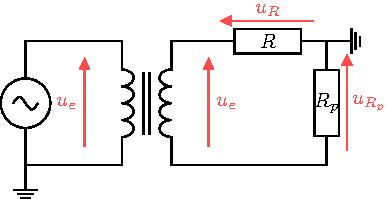
\includegraphics[width=\linewidth]{carac_r_oscillo}
			\captionof{figure}{}
			\label{fig:transfo}
		\end{center}
	\end{tcb}
}%

\setlist[blocQR,1]{leftmargin=10pt, label=\clenumi}
\QR<[start=5]>{%
	Retracer le circuit ci-contre, en enlevant le transformateur. La masse
	étant imposée par le générateur, proposer des branchements et
	manipulations pour observer $u_{R_p}$ sur la voie 1 et $u_R$ sur la
	voie 2.
}{%
	solu
}%

\QR{%
	Faire de même avec le circuit de la Figure~\ref{fig:transfo}. Conclure.
}{%
	solu
}%

\enonce{%
	\begin{tcb}(expe)<itc>{Tracé d'une caractéristique}
		\begin{enumerate}
			\item Réaliser le montage précédent en utilisant le GBF, avec $f =
				      \SI{1}{kHz}$, \texttt{level} $\approx \SIrange{2}{3}{V}$, sans
			      offset, $R_P = \SI{100}{\ohm}$ et $R$ \textit{inconnue}.
			\item Observer les 2 tensions à l'oscilloscope en centrant les deux voies.
		\end{enumerate}
	\end{tcb}
}%

\setlist[blocQR,1]{leftmargin=10pt, label=\sqenumi}
\QR<[start=6]>{%
	Visualise-t-on $u_{R_p}$ sans problème~? Que faut-il faire~?
}{%
	solu
}%

\QR{%
	Imprimer les deux courbes en prenant \textbf{le même gain vertical}, et
	\textbf{en déduire $R_{\rm inconnue}$}.
}{%
	solu
}%

\enonce{%
	\begin{tcb}(expe)<itc>{Mode XY}
		\begin{itemize}
			\item Dans le menu \texttt{horizontal}, passer en mode \texttt{XY}. On
			      visualise alors \texttt{CH2} en fonction de \texttt{CH1}, soit $u_R$
			      en fonction de $u_{R_p}$.
		\end{itemize}
	\end{tcb}
}%

\QR{%
	Que représente cette courbe~? La figer avec le bouton \texttt{STOP} et
	l'imprimer.
}{%
	solu
}%

\QR{%
	En déduire la valeur de $R_{\rm inconnue}$ avec une autre méthode que
	précédemment.
}{%
	solu
}%

\QR{%
	Conclure sur leur compatibilité grâce à un écart normalisé.
}{%
	solu
}%

\enonce{%
	\begin{tcb}(rema)<lfnt>{}
		Pour prendre l'opposé d'un signal, dans le menu de la voie presser
		\faIcon{arrow-down}, puis activer \texttt{Inversée}.
	\end{tcb}
}%

% \section{Réaliser~: Résistances d'entrée et de sortie}
% \subsection{Mesure de la résistance de sortie du GBF}
%
% \begin{enumerate}
% 	\item Réaliser le montage vu dans la partie \textit{S'approprier} pour une
% 	      fréquence d'environ $\SI{100}{Hz}$ et commencer avec $R'$ infinie, donc
% 	      débranchée.
% 	\item Mesurer alors $U_1$ grâce à l'oscilloscope, et régler le
% 	      \texttt{level} du GBF (bouton DC offset enfoncé) pour obtenir une
% 	      tension crête-crête de $\SI{2}{V}$. Cette tension correspond à la
% 	      tension à vide $e$ du générateur. En effet, à vide, c'est-à-dire pour
% 	      $R'$ infinie, le courant est nul et donc la tension relevée est
% 	      directement égale à $e$.
% 	\item Brancher la boîte de résistances variables $R'$ et l'ajuster pour
% 	      avoir $U_1 = e/2$.
% 	\item En déduire l'ordre de grandeur de la résistance de sortie $r_{s}$ du
% 	      GBF.
% 	\item Cette valeur est-elle cohérente avec les indications inscrites sur la
% 	      sortie du GBF~?
% \end{enumerate}
%
% \vspace{-0.6cm}
%
% \subsection{Mesure de la résistance d'entrée de l'oscilloscope (modèle)}
%
% \begin{enumerate}
% 	\item Prendre la notice de l'oscilloscope dont vous disposez, vérifier les
% 	      valeurs de $R_{e}$ et $C_{e}$ appelées \textit{input impedance} en
% 	      anglais.
% 	\item Mesurer d'abord la tension $U_{e}$ en connectant directement
% 	      l'oscilloscope au générateur (cela revient à prendre une résistance $R'$
% 	      nulle, assimilable à un fil donc).
% 	\item Réaliser ensuite le montage présenté dans la partie
% 	      \textit{S'approprier}.
% 	\item $U_{e}$ étant fixé ($\SI{2}{V}$ crête-crête), faire varier $R'$
% 	      jusqu'à ce que la tension aux bornes de l'oscilloscope ($U_2$) soit
% 	      égale à la moitié de la tension du générateur $U_{e}$. Vous pouvez
% 	      utiliser le menu mesure pour obtenir la valeur des deux tensions.
% 	\item En déduire l'ordre de grandeur de la résistance d'entrée $R_{e}$
% 	      expérimentale de l'oscilloscope.
% \end{enumerate}
%
\section{Valider} %~: Effets des résistances d'entrée et de sortie}
\subsection{Effet de la résistance de sortie du GBF}

\enonce{%
	\noindent
	\begin{minipage}[c]{.70\linewidth}
		Brancher l'oscilloscope aux bornes du GBF (toujours réglé à une fréquence de
		$\SI{1}{kHz}$) et régler le \texttt{level} de celui-ci pour obtenir une tension
		crête-crête de $\SI{2}{V}$. Comme précédemment, nous mesurons ici la tension à
		vide $e$ du GBF.
	\end{minipage}
	\hfill
	\begin{minipage}[c]{.25\linewidth}
		\begin{center}
			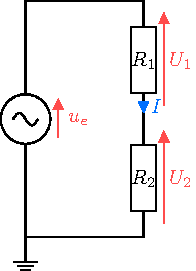
\includegraphics[width=.8\linewidth, rotate=90]{divis_tension}
			\captionof{figure}{}
		\end{center}
	\end{minipage}
}%

\QR{%
	Brancher aux bornes du GBF deux résistances identiques de
	$R_1 = R_2 = \SI{47}{\Omega}$ en série. Faire un schéma, puis relever
	à l'aide de l'oscilloscope la tension $U_2$ aux bornes de $R_2$.
}{%
	solu
}%

\QR{%
	En appliquant le principe du pont diviseur de tension, que devrait
	valoir $U_2$~? Est-ce la valeur que vous relevez~?
}{%
	solu
}%

\QR{%
	Expliquez cet écart en considérant la résistance de sortie du GBF.
}{%
	solu
}%

\QR{%
	Comment choisir $R_1$ et $R_2$ pour que l'on puisse négliger l'effet
	de la résistance de sortie du GBF~? Reproduire le montage précédent en
	utilisant désormais $R_1 = R_2 = \SI{10}{k\Omega}$. Montrer qu'alors
	$U_1$ prend la valeur attendue.
}{%
	solu
}%

\QR{%
	Pourrait-on brancher l’oscilloscope aux bornes de $R_1$~? Justifier.
}{%
	solu
}%

\subsection{Effet de la résistance d'entrée de l'oscilloscope}

\QR{%
	Brancher l'oscilloscope aux bornes du GBF (toujours réglé à une
	fréquence de $\SI{1}{kHz}$) et régler le \texttt{level} de celui-ci
	pour obtenir une tension crête-crête de $\SI{4}{V}$. Comme précédemment,
	nous mesurons ici la tension à vide $e$ du GBF.
}{%
	solu
}%

\QR{%
	Brancher aux bornes du GBF deux résistances identiques de $R_1 = R_2 =
		\SI{1}{M\Omega}$ en série puis relever à l'aide de l'oscilloscope la
	tension $U_1$ aux bornes de l'une d'elle.
}{%
	solu
}%

\QR{%
	La tension $U_1$ obtenue est-elle conforme à vos attentes~? Expliquez
	cet écart en tenant compte de la résistance d'entrée de l'oscilloscope.
}{%
	solu
}%

\QR{%
	Comment choisir $R_1$ et $R_2$ pour que l'on puisse négliger l'effet de
	la résistance d'entrée de l'oscilloscope~? Reproduire le montage
	précédent en utilisant désormais $R_1 = R_2 = \SI{10}{k\Omega}$. Montrer
	qu'alors $U_1$ prend la valeur attendue.
}{%
	solu
}%

\section{Conclure}

\QR{%
	Résumer les recommandations pratiques que vous avez pu déduire de ce TP
	afin de réaliser des mesures correctes en électricité.
}{%
	solu
}%

\end{document}
